\section{Questionnaire result}




The questionnaire remained open for a week, during which time it garnered responses from a total of 136 anonymous participants.
Since we shared the link out to friends and family, we are expecting the age distribution of the participants to be mainly around 18 to 25, with some participants reaching age 50 and above.
From our friend groups and family members, we assume all the participants to the questionnaire has basic knowledge to technology, such as navigate through websites or using social media.

\begin{figure}[ht]
  \centering
  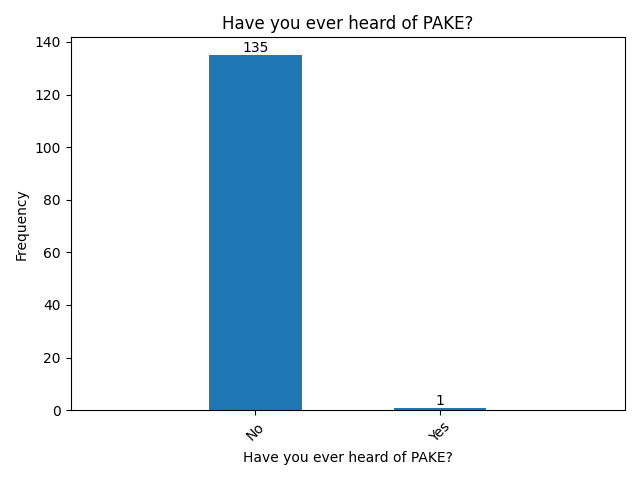
\includegraphics[width=0.4\textwidth]{./images/know_pake.png}
  \caption{Numbers of participants heard about PAKE}
  \label{fig:know_pake}
\end{figure}

\subsection{Knowledge about PAKE}
We asked the participants whether they have heard about PAKE protocols or not.
Initially, we did not expect any participants to know anything about PAKE, speaking from our experience that none of us knew PAKE until we start working on the project.
But surprisingly, one participant out of 136 actually knew about PAKE protocols with prior knowledge, as shown in ~\figref{fig:know_pake}.
They highlighted that "PAKE protocols use zero-knowledge proofs to authenticate without transmitting passwords. Good for security," which is the goal PAKE is aiming to achieve.





\begin{figure}[ht]
  \centering
  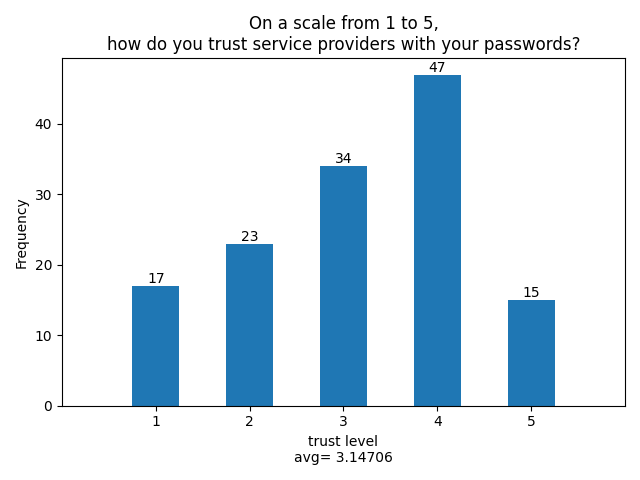
\includegraphics[width=0.4\textwidth]{./images/service_provider_trust.png}
  \caption{Trust towards service providers with participants' passwords.
    The intensity is measured on a scale of 1 to 5, where 1 represents not secure, and 5 represents very secure.}
  \label{fig:trust}
\end{figure}


\subsection{Trust to Password over TLS and service providers}
\label{sec:trust}
We are also curious how users trust service providers with their password.
We informed the participants that Password over TLS implementation requires storing encrypted password in the service providers' databases, and wanted to collect some feedback for this implementation.
Most answers surrounded the idea of data breach and leaks, which is one way an adversary gain control of a user's account.
One participant mentioned that "widely-used authentication methods, once subject to a data breach, are completely vulnerable: all users' data can be extracted, as user passwords are entirely stored on the server side databases."
While this is not entirely correct, storing password in server's database can add additional risks to lose all other personal data stored with the service provider.

Another participant mentioned password reusing, saying that most people would not bother to remember multiple passwords to different services, which can put all the services that use same password in danger if one of them is breached.
He also said in order to prevent the incident from happening, users often use password managers or notebook applications to keep track their passwords, but the additional use of programs brings another vulnerability to the potential leak of passwords.

Furthermore, we asked the participants whether they trust service providers with their passwords.
The result in ~\figref{fig:trust} shows that part of the uses are confident about their password being handled safely by the service providers, but at the same time, another part of the participants felt uncertain about the situation.
We can see a slightly right skewed trend from the figure, but we believe it is not significant enough to show whether a user trust the server would safe their passwords securely or not.
% From the average of the result, we did not see any significant tendency whether a user trust or is skeptical of the Password over TLS implementation.



\begin{figure}[ht]
  \centering
  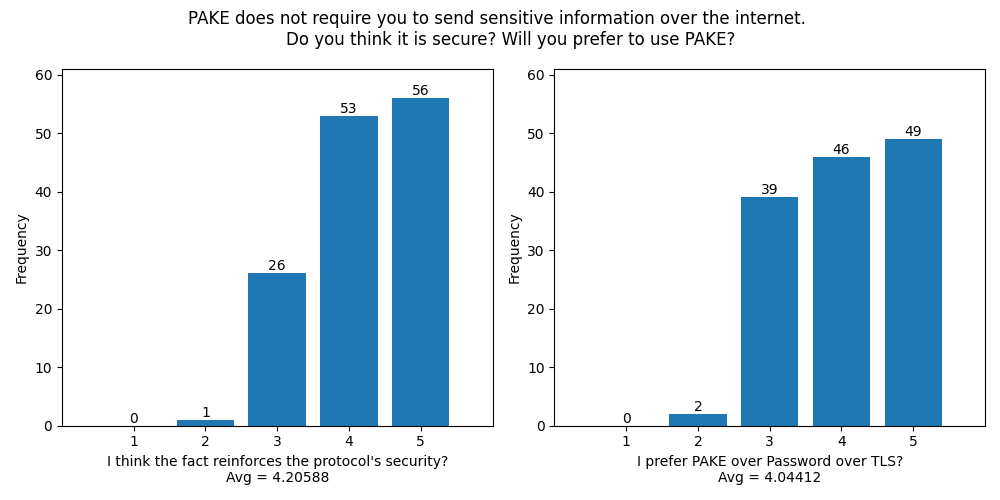
\includegraphics[width=0.4\textwidth]{./images/secure_preference.png}
  \caption{Participants' opinion on PAKE protocols. 
  The intensity is measured on a scale from 1 to 5, where 1 represents most unlikely, and 5 represents most likely}
  \label{fig:preference}
\end{figure}

\subsection{Preference between PAKE and Password over TLS}
\label{sec:preference}

In the questionnaire we stressed the point that PAKE protocols do not require passwords to be sent through the internet.
We would like to see how participants would response with this information, whether they think it is more secure or less.
From ~\figref{fig:preference}, it is apparent that the majority of participants view authentication methods that avoid transmitting passwords over the internet as more secure, and have a higher preference to embrace protocols that does not require transmitting.
% We can see such tendency are positively related to each other, 

In ~\secref{sec:trust}, participants pointed out some potential flaws Password over TLS have, but only a slight right skew on ~\figref{fig:trust} is observed.
% does not seem to have a common agreement on the trust towards service providers.
However, in ~\secref{sec:preference}, they showed high interest in using protocols that does not send sensitive information. 
We assume that the slight right skew comes from the trust towards big companies that most users think are reliable, but when an alternative that does not require sensitive data to be transmitted, users would opt for the second option to guard their security.

\begin{figure}[ht]
  \centering
  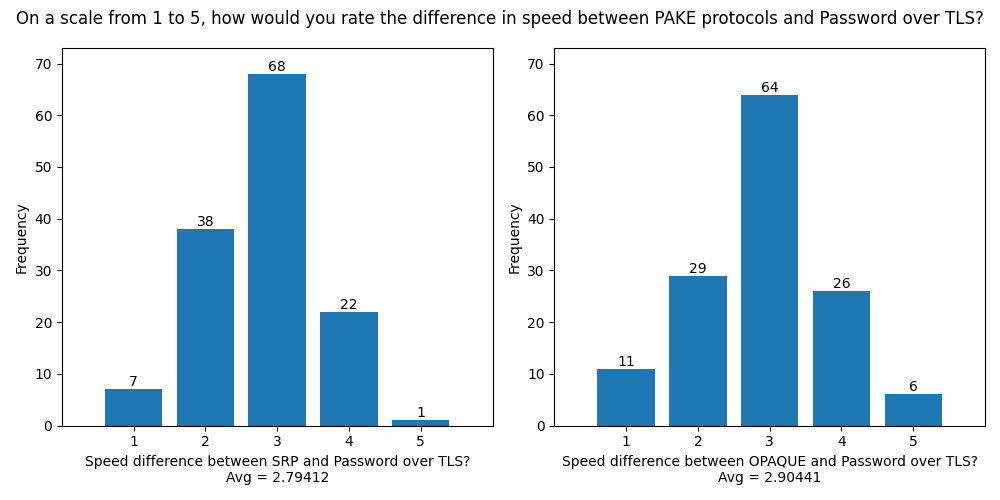
\includegraphics[width=0.4\textwidth]{./images/ux_compare.png}
  \caption{Response time difference between PAKE protocols and Password over TLS.
  The intensity is measured on a scale from 1 to 5, where 1 represents much slower, and 5 represents much faster.}
  \label{fig:compare}
\end{figure}

\subsection{User experience analysis}
We provided participants with access to the three implementations, enabling them to directly assess the variations in time consumption. 
Participants were then instructed to log in using all three services, assess their responsiveness, and make comparisons between the two PAKE protocols and the controlled Password over TLS implementation.
From ~\figref{fig:compare}, participants report similar time consumption when comparing both PAKE protocols to Password over TLS.

This raises our question about why PAKE is rarely implemented. 
Despite the minimal differences in user experience compared to Password over TLS, we anticipated increased adoption of PAKE across various platforms.
However, the reality contradicts our expectations.
We assume that developers chose not to implement PAKE protocols becuase the heavy workload that falls on the server side, showed in ~\secref{sec:exp_results}.
Also, PAKE implementations are much more complicated then Password over TLS, which requires much more effort to trace the logic when building the protocol and maintaining the system. 